\documentclass{article}
\usepackage{amsmath}
\usepackage{amssymb}
\usepackage{enumitem}
\usepackage{algorithm}
\usepackage{color}
\usepackage[table]{xcolor}
\usepackage[T1]{fontenc}
\usepackage{etoolbox}
\usepackage{multicol}
\usepackage{multirow}
\usepackage{fancyhdr}
\usepackage{graphicx}
\usepackage{array}
\usepackage{animate}
\usepackage{amsthm}
\usepackage{caption}
\usepackage{minted}
\usepackage{geometry}
\usepackage{tikz, pgfplots, tkz-euclide,calc}
    \usetikzlibrary{patterns,snakes,shapes.arrows,shapes.geometric,arrows}
    \geometry{
        total = {160mm, 237mm},
        left = 35mm,
        right = 35mm,
        top = 40mm,
        bottom = 40mm,
        headheight=2cm
      }
\usepackage{hyperref}
\hypersetup{
    colorlinks=true,
    linkcolor=blue,
    filecolor=magenta,      
    urlcolor=cyan,
    pdftitle={Overleaf Example},
    pdfpagemode=FullScreen,
    }

\newcommand{\enter}{\raisebox{-1.8pt}{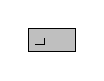
\begin{tikzpicture}[scale=0.3]
    \draw[thin,fill=lightgray] (0,0) rectangle (2,1);
    \draw (0.3,0.3) -- (0.7,0.3)--(0.7,0.6);     
\end{tikzpicture}}}

\definecolor{HIMAmuda}{HTML}{01D1FD}
\definecolor{HIMAtua}{HTML}{02016A}
\definecolor{HIMAabu}{HTML}{CBCBCC}
\definecolor{pgray}{rgb}{0.5,0.5,0.5}
\definecolor{pblue}{rgb}{0.13,0.13,1}
\definecolor{pgreen}{rgb}{0,0.5,0}
\definecolor{pred}{rgb}{0.9,0,0}
\definecolor{pgrey}{rgb}{0.46,0.45,0.48}
\definecolor{pcyan}{HTML}{D4EFFC}
\definecolor{lblue}{HTML}{00AEEF}
\definecolor{input}{HTML}{AAE1FA}
\definecolor{bg}{rgb}{0.95, 0.95, 0.92}
\definecolor{vscode}{HTML}{282A36}
\definecolor{PastelGreen}{HTML}{77DD77}

\tikzstyle{startstop} = [rectangle, rounded corners, 
minimum width=2cm, 
minimum height=1cm,
text centered, 
draw=black, 
fill=pink]

\tikzstyle{io} = [trapezium, 
trapezium stretches=true, % A later addition
trapezium left angle=70, 
trapezium right angle=110, 
minimum width=2cm, 
minimum height=1cm, text centered, 
draw=black, fill=HIMAmuda]

\tikzstyle{process} = [rectangle, 
minimum width=1cm, 
minimum height=1cm, 
text centered, 
text width=2.5cm, 
draw=black, 
fill=HIMAabu]

\tikzstyle{decision} = [diamond, 
minimum width=1cm, 
minimum height=1cm, 
text width=1.3cm, 
text centered, 
draw=black, 
fill=PastelGreen]
\tikzstyle{arrow} = [thick,->,>=stealth]

\newcommand{\inputscan}[1]{\raisebox{0pt}[1pt]{\colorbox{darkgray}{#1}}}

\usepackage{listings}

\lstdefinestyle{standard}{
    language            = Java,
    showspaces          = false,
    showtabs            = false,
    breaklines          = true,
    showstringspaces    = false,
    breakatwhitespace   = true,
    commentstyle        = \color{pgray},
    keywordstyle        = \color{pblue},
    stringstyle         = \color{pgreen},
    basicstyle          = \footnotesize\ttfamily,
    frame               = single,
    backgroundcolor     = \color{brown!10!white},
    escapeinside        = {(*}{*)},
    numbers             = left, % {none, left, right}
    numberstyle         = \scriptsize\color{lightgray},
    numbersep           = -8pt,
    }

\lstdefinestyle{output}{
    language=Java,
    backgroundcolor     =\color{vscode},
    basicstyle          =\footnotesize\ttfamily\color{white},
    frame               =shadowbox,
    escapeinside        ={(*}{*)},
    showspaces          =false,
    showtabs            =false,
    breaklines          =true,
    showstringspaces    =false,
    breakatwhitespace   =true,
    rulesepcolor        =\color{HIMAtua!50!white},
    rulecolor           =\color{HIMAtua!50!white},
    numbers             =none,
    }

\lstdefinestyle{soal}{
    language=Java,
    basicstyle=\ttfamily\small,
    keywordstyle=\color{blue}\bfseries,
    commentstyle=\color{gray},
    stringstyle=\color{red},
    numbers=left,                     % Menampilkan nomor baris
    numberstyle=\tiny\color{gray},    % Ukuran dan warna nomor baris
    stepnumber=1,                     % Menampilkan nomor baris setiap baris
    numbersep=5pt,                    % Jarak antara nomor baris dan teks
    backgroundcolor=\color{white},    % Warna latar belakang
    showspaces=false,                 % Jangan tampilkan spasi
    showstringspaces=false,           % Jangan tampilkan spasi di dalam string
    showtabs=false,                   % Jangan tampilkan karakter tab
    frame=single,                     % Bingkai di sekitar kode
    tabsize=4,                        % Ukuran tab
    captionpos=b,                     % Posisi caption (b=bottom, t=top)
    breaklines=true,                  % Membungkus baris yang panjang
    breakatwhitespace=false,          % Membungkus di whitespace
    escapeinside={(*}{*)}            % Escape dari LaTeX dalam kode
}

\lstset{style=standard}

\graphicspath{{C:/Users/teoso/OneDrive/Documents/Tugas Kuliah/Template Math Depart/}}

\newcommand{\R}{\mathbb{R}}
\newcommand{\N}{\mathbb{N}}
\newcommand{\Z}{\mathbb{Z}}
\newcommand{\Q}{\mathbb{Q}}
\newcommand{\jawab}{\textbf{Solusi}:}

\newtheorem*{teorema}{Teorema}
\newtheorem*{definisi}{Definisi}

\renewcommand{\headrulewidth}{0pt}
\renewcommand{\figurename}{Gambar}
\renewcommand{\tablename}{Tabel}

\begin{document}
\fancyhead[C]{
\begin{tabular}{l c  r}
    \multirow{4}{3cm}{\includegraphics[width=1.3cm]{ITS.png}}
    &\textbf{\MakeUppercase{evaluasi tengah semester}}&\multirow{4}{3cm}{\raggedleft\includegraphics[width=1.3cm]{M.png}}\\
    &\textbf{\MakeUppercase{semester ganjil 2024/2025}}&\\
    &\textbf{\MakeUppercase{departemen matematika - fsad its}}&\\
    &\textbf{\MakeUppercase{program sarjana}}&\\
\end{tabular}}
\pagestyle{fancy}

\indent
\textbf{Aturan Pengerjaan:}
\begin{itemize}
    \item Dilarang bekerja sama dalam bentuk apa pun. Segala jenis pelanggaran (mencontek, kerjasama, dsb) yang dilakukan saat ETS akan dikenakan sanksi pembatalan mata kuliah pada semester yang sedang berjalan.
    \item Tuliskan Pakta Integritas di awal lembar jawaban Anda, sebagai berikut: ``Dengan ini saya menyatakan bahwa saya mengerjakan sendiri tanpa bantuan dan membantu orang lain dalam menyelesaikan soal-soal ETS Alpro 1'' dan ditandatangani.
\end{itemize}

\noindent
Kerjakan soal-soal berikut dengan sejelas-jelasnya!
\begin{enumerate}
    \item \textbf{(Skor: 20)} Lengkapi program Java berikut ini, agar program berfungsi untuk menentukan apakah sebuah bilangan bulat positif $n$ yang diinputkan oleh pengguna adalah bilangan prima atau bukan. Suatu bilangan prima hanya habis dibagi 1 dan bilangan itu sendiri. Sebelum melengkapi program, buatlah flowchartnya terlebih dahulu.
    \begin{minted}[fontsize=\footnotesize,frame=lines,
        framesep=2mm,linenos]{java}
import java.util.Scanner;
public class bilPrima {
    public static void main(String[] args) {
        Scanner inp = new Scanner(System.in);
        System.out.print("Masukkan bilangan: ");
        int n = inp.nextInt();
    
        boolean isPrima = true;
        
        ...
        
        if (isPrima) {
            System.out.println(n + " adalah bilangan prima.");
        } else {
            System.out.println(n + " bukan bilangan prima.");
        }
    }
}
    \end{minted}
    \begin{flushright}
        (\textit{Bandung Arry Sanjoyo})
    \end{flushright}

    \item \textbf{(Skor: 20)} Tuliskan (dan telusuri) sebuah program Java yang inputnya berupa sebuah bilangan bulat yang diinput oleh user melalui keyboard, dan menghasilkan output berupa jumlah angka-angka dasar yang gasal dari bilangan input tersebut. Sebagai contoh, jika user memberi input bilangan nonnegatif, misal $23032$, maka akan tercetak:

    \begin{quote}
        \centering
        \texttt{Jumlah angka dasar gasal dari 23032 adalah 6}
    \end{quote}

    Sedangkan jika user memberi input bilangan negatif, misal $-54321$, maka akan tercetak:

    \begin{quote}
        \centering
        \texttt{Jumlah angka dasar gasal dari -54321 adalah 9}
    \end{quote}

    \begin{flushright}
        (\textit{Nurul Hidayat})
    \end{flushright}
    
    \item \textbf{(Skor: 20)} Perhitungan BMI (\textit{Body Mass Index}) digunakan sebagai salah satu ukuran kesehatan berdasarkan berat badan (kilogram) dan tinggi badan (meter), dengan rumus:
    \[
    \text{BMI} = \frac{\text{Berat badan}}{\text{tinggi badan}^2}
    \]
    
    Berikut klasifikasi BMI beserta keterangan risikonya:
    \begin{table}[h!]
        \centering
        \begin{tabular}{|m{3.5cm}|c|m{4.5cm}|}
            \hline
            \rowcolor{input}
            \textbf{Klasifikasi} & \textbf{BMI (kg/m\(^2\))} & \textbf{Risiko Komorbiditas} \\
            \hline
            \raggedright Berat badan kurang & $<$ 18,5 & Rendah (tapi risiko masalah klinis lain meningkat) \\
            \hline
            \raggedright Berat badan ideal & 18,5 -- 22,9 & Rata-rata \\
            \hline
            \raggedright Berat badan berlebih (overweight) & 23,0 -- 24,9 & Meningkat \\
            \hline
            Obesitas tingkat 1 & 25,0 -- 29,9 & Sedang \\
            \hline
            Obesitas tingkat 2 & $\geq$ 30,0 & Berat \\
            \hline
        \end{tabular}
        \caption{Tabel Klasifikasi BMI}
    \end{table}

    Buat program Java yang dapat menghitung nilai BMI dengan menggunakan \texttt{if-else if}.
    
    Contoh keluaran program:\\
    \texttt{Berat Badan Anda (kg): 60} \\
    \texttt{Tinggi Badan Anda (m): 1.6} \\
    \texttt{BMI Anda: 23.437499999999996} \\
    \texttt{Risiko Anda: Meningkat}

    \begin{flushright}
        (\textit{Alvida Mustika Tukmi})
    \end{flushright}

    \item \textbf{(Skor: 20)} Perhatikan program berikut!

    \begin{minted}[fontsize=\footnotesize,frame=lines,
        framesep=2mm,linenos]{java}
import java.util.Scanner;

public class ETSSelections {
    public static void main(String[] args) {
        Scanner input = new Scanner(System.in);
    
        System.out.print("Masukkan bilangan tiga digit: ");
        int number = input.nextInt();
    
        int digit1 = (int)(number / 100);
        int remaining = number % 100;
        int digit3 = (int)(remaining % 10);
    
        System.out.println(
            number + ((digit1 == digit3) ? 
            " merupakan " : " bukan merupakan ") + "palindrom");
    }
}

    \end{minted}
    \begin{enumerate}
        \item Telusuri program tersebut dan jelaskan apa yang dicetak dari program tersebut!
        \item Tuliskan ulang sintaks program di atas dengan mengganti baris 16 dengan operator \texttt{if-else}.
    \end{enumerate}

    \textbf{Keterangan:} Telusuri program berarti Anda diminta untuk menjelaskan proses dari program tersebut.
    
    \begin{flushright}
    \textit{(Raden Aurelius Andhika Viadinugroho)}
    \end{flushright}
    
    \item \textbf{(Skor: 20)} Dalam metode statistika, dikenal ukuran pemusatan dan ukuran penyebaran, diantaranya adalah mean dan standar deviasi. Keterangan dari ukuran-ukuran tersebut adalah sebagai berikut:
    
    \begin{itemize}
        \item Mean mengukur rata-rata dari data yang diberikan, dengan persamaan dari mean adalah:
        \[
        \bar{x} = \frac{\sum_{i=1}^{n} x_i}{n} = \frac{x_1 + x_2 + \cdots + x_n}{n}
        \]
        dengan $\bar{x}$ adalah mean dan $x_i$ adalah observasi ke-$i$ dari data.
        
        \item Standar deviasi adalah ukuran statistik yang mengukur sebaran dari data. Persamaan dari standar deviasi adalah:
        \[
        s = \sqrt{\frac{\sum_{i=1}^{n} (x_i - \bar{x})^2}{n - 1}} = \sqrt{\frac{\sum_{i=1}^{n} x_i^2}{n - 1} - \frac{\left( \sum_{i=1}^{n} x_i \right)^2}{n(n-1)}}
        \]
    \end{itemize}
    
    Berdasarkan informasi di atas, buatlah program dalam bahasa Java yang dapat membaca input berupa jumlah data yang diinginkan dan bilangan sebagai observasi data sesuai dengan jumlah data yang diinginkan dan mengeluarkan output berupa mean dan standar deviasi dari bilangan yang diinputkan. Telusuri program yang Anda buat!
    
    \textbf{Hint:} Sebagai contoh, misal jumlah data yang diinginkan adalah 10, maka ada 10 bilangan yang perlu diinput untuk dihitung mean dan standar deviasinya.
    
    \begin{flushright}
    \textit{(Raden Aurelius Andhika Viadinugroho)}
    \end{flushright}
    
\end{enumerate}

    \begin{center}
        \textbf{SELAMAT MENGERJAKAN}
    \end{center}

    \newpage
    \fancyhead[C]{
\begin{tabular}{l c  r}
    \multirow{3}{2cm}{\includegraphics[width=1.3cm]{Provicom.png}}
    &\textbf{\MakeUppercase{Pembahasan ETS}}&\multirow{3}{2cm}{\raggedleft\includegraphics[width=1.5cm]{provicomIG.png}}\\
    &\textbf{\MakeUppercase{Asisten laboratorium}}&\\
    &\textbf{\MakeUppercase{Lab. pemrograman dan komputasi visual}}&\\
\end{tabular}}
    \begin{enumerate}
        \item Definisi yang telah diberikan di soal tentang bilangan prima adalah ``suatu bilangan prima hanya habis dibagi 1 dan bilangan itu sendiri''. Hal ini bisa kita buat pernyataan yang ekivalen yaitu {\color{red}``suatu bilangan prima tidak habis dibagi oleh bilangan diantara rentang 1 sampai bilangan itu sendiri''}. Untuk bilangan prima, biasanya kita batasi inputnya untuk $n\geq 2$.
        \begin{figure}[h!]
            \centering
            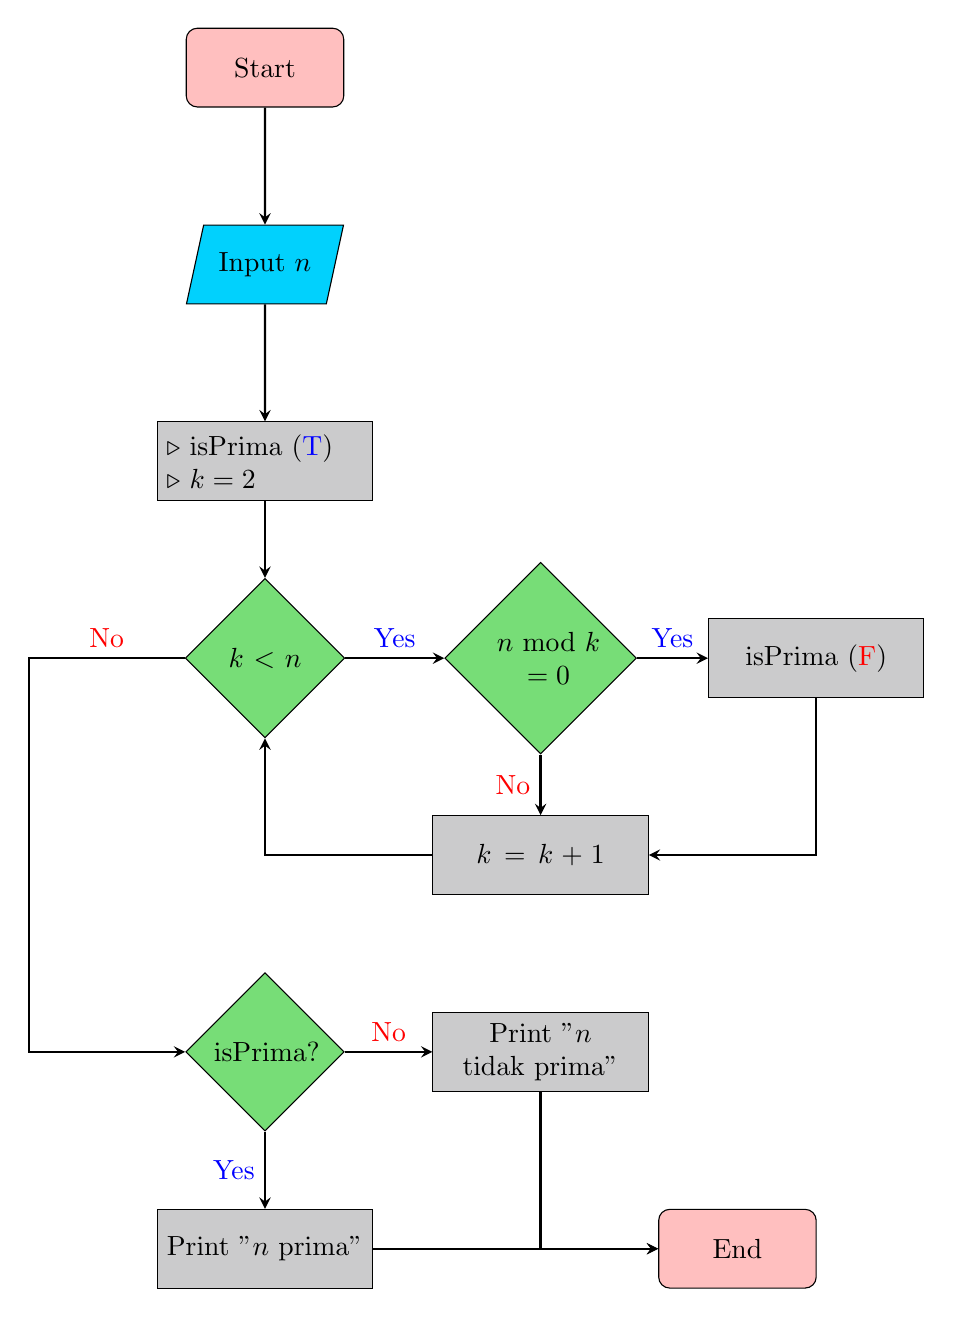
\begin{tikzpicture}[node distance=2.5cm]
                \node[startstop] (start) {Start};
                \node[io, below of=start] (inp) {Input $n$};
                \node[process, below of=inp] (init) {\parbox{2.5cm}{$\triangleright$ isPrima ({\color{blue}T})\\
                $\triangleright$ $k=2$
                }};
                \node[decision, below of=init] (loop) {$k < n$};
                \node[decision, right of=loop, xshift=1cm] (div) {\parbox{1.5cm}{\centering$n\text{ mod } k$\\$=0$}};
                \node[process, right of=div,xshift=1cm] (notPrima) {isPrima ({\color{red}F})};
                \node[process, below of=div] (inc) {$k=k+1$};
                \node[decision, below of=loop,yshift=-2.5cm] (YoN) {isPrima?}; 
                \node[process, below of=YoN] (P) {Print "$n$ prima"}; 
                \node[process, right of=YoN,xshift=1cm] (nP) {Print "$n$ tidak prima"}; 
                \node[startstop, below of=nP,xshift=2.5cm] (end) {End};

                \draw[arrow] (start) -- (inp);
                \draw[arrow] (inp) -- (init);
                \draw[arrow] (init) -- (loop);
                \draw[arrow] (loop) -- node[anchor=south] {\color{blue}Yes} (div);
                \draw[arrow] (div) -- node[anchor=south] {\color{blue}Yes} (notPrima);
                \draw[arrow] (div) -- node[anchor=east] {\color{red}No} (inc);
                \draw[arrow] (notPrima) |- (inc);
                \draw[arrow] (inc) -| (loop);
                \draw[arrow] (loop) -- node[anchor=south] {\color{red}No} ++(-3,0) |- (YoN);
                \draw[arrow] (YoN) -- node[anchor=east] {\color{blue}Yes} (P);
                \draw[arrow] (YoN) -- node[anchor=south] {\color{red}No} (nP);
                \draw[arrow] (nP) |- (end);
                \draw[arrow] (P) -- (end);
            \end{tikzpicture}
            \caption{Flowchart Program Bilangan Prima}
        \end{figure}\\
        Ada banyak cara untuk melengkapi program yang diberikan, misalnya menggunakan loop \texttt{for}, \texttt{while}, maupun \texttt{do-while}. Berikut adalah dua cara untuk melengkapi program tersebut:\footnote{Jika ada program yang lebih efektif atau lebih singkat, silahkan bisa menuliskan program tersebut saja. Misalkan kita ``bataskan nilai $k$ hingga menuju $\sqrt{n}$'' atau ``loop berhenti ketika \texttt{isPrima = false}'' }
        \begin{minted}[frame=lines,
            framesep=2mm,
            baselinestretch=1.2,
            bgcolor=bg,
            fontsize=\footnotesize,
            linenos]{java}
    int k = 2;
    while (k<n) {
        if (n % k == 0) {
            isPrima = false;
        }
        k++;
    }
        \end{minted}
        \begin{minted}[frame=lines,
            framesep=2mm,
            baselinestretch=1.2,
            bgcolor=bg,
            fontsize=\footnotesize,
            linenos]{java}
    for (int k = 2; k < n ; k++) {
        if (n % k == 0) {
            isPrima = false;
        }
    }   
        \end{minted}
        \begin{flushright}
            (\textit{Farvez, Jiryan, Tetew})
        \end{flushright}

        \item Pada contoh \textit{output} pada soal, kita perlu mempertimbangkan bilangan bulat negatif, sebab ketika dimodulokan akan menghasilkan bilangan yang negatif juga. Oleh karena itu, kita perlu mengubah bilangan negatif menjadi positif.\\
        
        Terdapat 2 cara untuk mengubah bilangan negatif menjadi positif, yaitu dengan menggunakan \texttt{Math.abs()}\footnote{Ingat bahwa \texttt{Math.abs()} menghasilkan bilangan \texttt{double}, sehingga untuk lebih amannya bisa di-\textit{casting} menjadi \texttt{int}} atau dengan menggunakan kondisi \texttt{if(n < 0) {n = -n;}}\\

        Langkah-langkah dalam programnya adalah sebagai berikut:
        \begin{enumerate}[label=(\arabic*)]
            \item Menerima input bilangan dari pengguna.
            \item Jika negatif, bilangan tersebut diubah menjadi positif.
            \item Bilangan akan masuk kedalam loop dan akan diambil digit terakhirnya menggunakan $\mod 10$.
            \item Jika digit tersebut ganjil, maka jumlahkan digit tersebut pada sebuah variabel. Jika genap, maka abaikan.
            \item Bilangan tersebut dibagi 10 untuk menghilangkan digit terakhirnya.(sifat dari \text{int})
            \item Ulangi langkah 3-5 hingga bilangan tersebut bernilai 0.
            \item Tampilkan jumlahan digit ganjil yang sudah disimpan dalam sebuah variabel.
        \end{enumerate}
        
        \inputminted[frame=lines,
        framesep=2mm,
        baselinestretch=1.2,
        bgcolor=bg,
        fontsize=\footnotesize,
        linenos]{java}{no2.java}
        \begin{flushright}
            (\textit{Farvez, Tetew})
        \end{flushright}
        
        \item Tidak ada cara khusus dalam membuat program ini, salah satu bentuk programnya adalah sebagai berikut:
        \inputminted[frame=lines,
        framesep=2mm,
        baselinestretch=1.2,
        bgcolor=bg,
        fontsize=\footnotesize,
        linenos]{java}{no3.java}
        \begin{flushright}
            (\textit{Farvez, Dios})
        \end{flushright}

        \item \begin{enumerate}
            \item Sebagai pengetahuan tambahan, kita lihat apa definisi dari \textit{palindrom}.
            \begin{definisi}
                Palindrom adalah sebuah kata, frasa, angka, atau urutan karakter yang dapat dibaca sama baik dari depan maupun dari belakang.
            \end{definisi}
            Karena program tersebut meminta 3 digit angka, maka program hanya perlu membandingkan digit pertama dengan digit ketiga. Kemudian terdapat \textit{ternary operator} dalam \texttt{System.out.println()} yang akan mencetak apakah bilangan tersebut palindrom atau tidak.

            \item Berikut adalah program yang telah diubah menggunakan \texttt{if-else}:
            \begin{minted}[frame=lines,
                framesep=2mm,
                baselinestretch=1.2,
                bgcolor=bg,
                fontsize=\footnotesize,
                linenos]{java}
        import java.util.Scanner;
        
        public class ETSSelections {
            public static void main(String[] args) {
                Scanner input = new Scanner(System.in);
            
                System.out.print("Masukkan bilangan tiga digit: ");
                int number = input.nextInt();
            
                int digit1 = (int)(number / 100);
                int remaining = number % 100;
                int digit3 = (int)(remaining % 10);
            
                if (digit1 == digit3) {
                System.out.println(number + " merupakan palindrom");
                } else {
                System.out.println(number + " bukan merupakan palindrom");
                }
            }
        }
            \end{minted}
        \end{enumerate}
        \begin{flushright}
            (\textit{Farvez, Dios, Tetew})
        \end{flushright}
        
        \item {\color{red}Jika sudah diajarkan tentang \texttt{array}, maka boleh mengunakan hal tersebut. Disini karena materi praktikum belum sampai \texttt{array}, maka kuasumsikan belum semuanya mempelajarinya}. Langkah-langkah membuat programnya adalah sebagai berikut:
        \begin{enumerate}[label=(\arabic*)]
            \item Meng-\textit{import} kelas \texttt{Scanner} dari pustaka \texttt{java.util}.
            \item Membuat kelas dan \textit{method} \texttt{main}.
            \item Membuat objek \texttt{Scanner} dengan nama \texttt{input}.
            \item Membuat variabel \texttt{n} bertipe data \texttt{int} untuk menyimpan jumlah data yang diinginkan.
            \item Menginisialisasi variabel \texttt{data}, \texttt{sum}, dan \texttt{sum\_2}.
            \item Membuat loop \texttt{for} untuk menginputkan data sebanyak \texttt{n} kali yang disimpan dalam variabel \texttt{data}.
            \item Didalam loop, tambahkan nilai \texttt{data} ke variabel \texttt{sum} dan \texttt{sum\_2}.
            \item Setelah loop selesai, hitung nilai mean dengan rumus \texttt{mean = sum / n}.
            \item Kemudian hitung nilai standar deviasi dengan rumus \texttt{s = Math.sqrt((sum\_2 - (sum*sum)/n) / (n-1))}.
            \item Tampilkan nilai $\bar{x}$ dan $s$ menggunakan \texttt{System.out.println()}.
        \end{enumerate}
        \inputminted[frame=lines,
        framesep=2mm,
        baselinestretch=1.2,
        bgcolor=bg,
        fontsize=\footnotesize,
        linenos]{java}{no5.java}
        Contoh output program:
        \begin{quote}
    \noindent\texttt{Masukkan jumlah data yang diinginkan: 10\\
    Masukkan 10 buah data:\\
    1 2 3 4 5 6 7 8 9 0\\
    Mean: 4.5\\
    Standar deviasi: 3.0276503540974917}
        \end{quote}
    \begin{flushright}
        (\textit{Tetew})
    \end{flushright}
    \end{enumerate}
    \begin{figure}[h!]
        \centering
        \caption*{\textbf{SELAMAT TELAH MELEWATI MASA ETS:D}}
        \animategraphics[autoplay,loop,width=0.3\textwidth]{30}{Kita Ikuyo Doodle/Kita Ikuyo Doodle-}{0}{85}
    \end{figure}
\end{document}
